\documentclass[onecolumn,a4paper,dvipdfmx]{ieicejsp}
\usepackage[T1]{fontenc}
\usepackage{lmodern}
\usepackage{textcomp}
\usepackage{latexsym}
\usepackage{float}
\usepackage{graphicx}
\usepackage{amsmath, amssymb}
\usepackage{bm}
\usepackage{upgreek}
\usepackage{caption}
\usepackage{subcaption}
\renewcommand{\thesubfigure}{\Alph{subfigure}}
\renewcommand{\thesubtable}{\Alph{subtable}}

\title{
    {\bf AI を用いたファインバブル発生装置の最適操作条件の検討}
    {\normalsize \\ Optimal Operating Condition Design for a Fine Bubble Generator Using AI }
}
\author{
    著者 \\ Author
}
\affliate{%
    湘南工科大学 AI R\&D Center \\
    Shonan Institute of Technology, AI R\&D Center\\
}

\begin{document}
\maketitle

\section{実験}
\label{sec_experiment}

\subsection{データの収集}
\label{sec_data_collection}

本研究では，ファインバブル（Fine Bubble，FB）発生装置 FBG-OS Type1 を用いてファインバブルを生成した．
実験系の概略を図\ref{fig_procedure}に示す．
酸素ボンベから供給される酸素と純水を HPLC ポンプおよび Air-Water Mixer で混合し，Dissolution Tubing を通過させて溶解槽に導入する．
溶解した気液混合流体は Discharge Tubing および Back Pressure Regulator を経て水温 30\,\textcelsius に保たれた Water Bath 内へ吐出され，FB 懸濁液として回収される．
回収した FB 懸濁液は 3-way stopcock を介して分取され，一部は Syringe Pump によって供給される純水を background として NanoSight LM10 に導入しナノバブル（Nanobubble，NB）濃度を測定した．
本稿では，NB の普及した呼称である UFB を用いて UFB 濃度（UFB conc.）と表記する．
また，別経路で PartAn SI にも導入し MB 濃度（MB conc.）を測定した．
生成された FB を含む水中の溶存酸素量（Oxygen content，Oxygen cont.）は Oxygraph により測定した．

本研究では，FB の生成条件を説明変数，生成された FB の物性値を目的変数として扱う．
ここで，説明変数とは目的変数を予測するために用いる変数であり，目的変数とは予測の対象となる変数である．

説明変数として設定した 6 つの因子とその設定水準を表\ref{tab_conditions}(A)に，本稿で扱う目的変数とその意味を表\ref{tab_conditions}(B)に示す．
これら 6 つの因子の組み合わせのうち 39 通りの操作条件について FB を生成し，各条件につき 1〜5 回の反復測定を行った結果，合計 82 サンプルのデータセットを構築した．
目的変数としては，UFB 濃度，MB 濃度，酸素含量に加えて，Mean size，Mode size，Size (bin) の計 6 種を測定したが，本稿で分析対象とする目的変数の選定については\ref{sec_condition}節で述べる．

\begin{table}[H]
    \caption{実験条件および目的変数の一覧}
    \vspace{2mm}
    \centering
    \begin{subtable}[t]{\linewidth}
        \centering
        \caption{説明変数と設定水準}
        \begin{tabular}{cc}
            \hline
            説明変数 & 設定水準 \\
            \hline
            溶解管長さ（Dissolve tube） & 0.12，2\,m \\
            溶解圧力（Dissolution pressure） & 2，3，4\,MPa \\
            吐出管長さ（Discharge tube） & 0.7，2，4，5\,m \\
            酸素流量（Flow speed (oxygen)） & 3.3，5，10，25\,mL/min \\
            水流量（Flow speed (water)） & 25，40，45，46.7\,mL/min \\
            水量（Water volume） & 50，100\,mL \\
            \hline
        \end{tabular}
        \label{tab_conditions_a}
    \end{subtable}

    \vspace{3mm}

    \begin{subtable}[t]{\linewidth}
        \centering
        \caption{目的変数とその意味}
        \begin{tabular}{cc}
            \hline
            目的変数 & 意味 \\
            \hline
            MB conc. & PartAn SI により測定した MB（Micro Bubble）濃度 \\
            UFB conc. & NanoSight LM10 により測定したナノバブル（Nanobubble）濃度 \\
            Oxygen cont. & Oxygraph により測定した溶存酸素量 \\
            \hline
        \end{tabular}
        \label{tab_conditions_b}
    \end{subtable}
    \label{tab_conditions}
\end{table}

\begin{figure}[H]
    \centering
    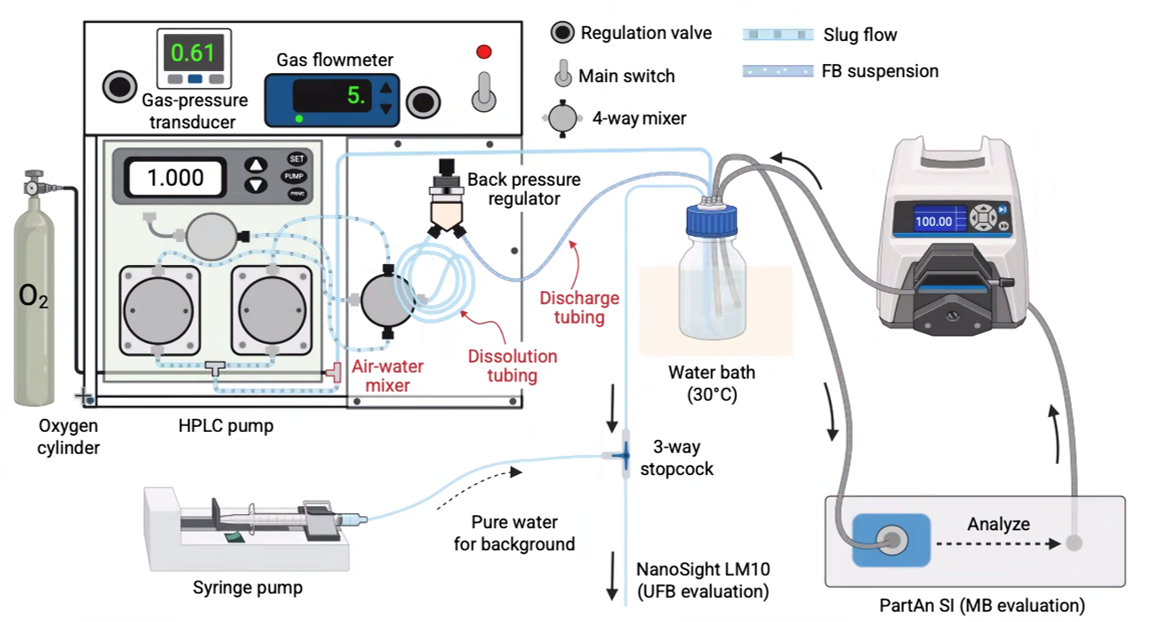
\includegraphics[width=0.7\linewidth]{figures/figure1_experimental_procedure.png}
    \caption{FB 発生・評価系の概略図}
    \label{fig_procedure}
\end{figure}

\subsection{実験条件}
\label{sec_condition}

目的変数は測定量ごとに単位およびスケールが異なるため，複数の目的変数を統一的な基準で比較するにあたり，各目的変数を式(\ref{eq_standardization})により標準化した．

\begin{equation}
    z_i^t = \frac{ y_i^t - \mu^t }{ \sigma^t }
    \label{eq_standardization}
\end{equation}

\noindent
ここで $ t $ は目的変数の種類（例えば $ t = \text{MB conc.} $），$ y_i^t $ は目的変数 $ t $ の $ i $ 番目のサンプルにおける標準化前の値，$ \mu^t $ は目的変数 $ t $ の全サンプルにおける平均，$ \sigma^t $ は同標準偏差，$ z_i^t $ は標準化後の値である．
以降で述べる変動係数および郡内標準偏差の算出，モデルの学習・評価は，すべてこの標準化後の値を用いて行った．

複数存在する目的変数の中から分析対象とすべき変数を選定する根拠として，変動係数（Coefficient of Variation，CV）と郡内標準偏差の 2 つの指標を用いた．
CV は式(\ref{eq_cv})の通り，目的変数 $ t $ の全サンプルにおける標準偏差 $ \sigma^t $ を平均 $ \mu^t $ で除した値であり，操作条件の違いを含めた目的変数全体の相対的なばらつきの大きさを表す．

\begin{equation}
    \mathrm{CV}^t = \frac{ \sigma^t }{ \mu^t }
    \label{eq_cv}
\end{equation}

一方，同一の操作条件で複数回測定した際のばらつきは，操作条件によらない測定・製造上の再現性誤差とみなせる．
そこで，同一の操作条件を 1 つの郡（group）とみなし，郡 $ k $（$ k = 1, \dots, G $）に属する目的変数 $ t $ の標準化後のサンプル $ z_{k,1}^t, \dots, z_{k,n_k}^t $（郡内サンプル数 $ n_k $，郡内平均 $ \bar{z}_k^t $）について式(\ref{eq_within_group_std_k})により郡内標準偏差 $ s_k^t $ を求め，式(\ref{eq_within_group_std})によりすべての郡について平均した値を郡内標準偏差 $ \bar{s}^t $ とした．
本データセットでは，操作条件の組み合わせ数は $ G = 39 $ である．

\begin{equation}
    s_k^t = \sqrt{ \frac{1}{n_k} \sum_{j=1}^{n_k} \left( z_{k,j}^t - \bar{z}_k^t \right)^2 }
    \label{eq_within_group_std_k}
\end{equation}

\begin{equation}
    \bar{s}^t = \frac{1}{G} \sum_{k=1}^{G} s_k^t
    \label{eq_within_group_std}
\end{equation}

CV が大きく，かつ郡内標準偏差が小さい目的変数ほど，操作条件の違いによる変動が測定誤差に比べて相対的に大きく，操作条件から目的変数を予測する回帰問題として妥当であるといえる．
表\ref{tab_cv}に，測定した 6 種の目的変数について算出した CV と郡内標準偏差を示す．
UFB 濃度（$ \mathrm{CV} = 0.636 $，$ \bar{s} = 0.349 $）および MB 濃度（$ \mathrm{CV} = 0.688 $，$ \bar{s} = 0.167 $）は，他の目的変数と比較して CV が大きく郡内標準偏差が小さいことから，操作条件によって系統的に変動しており，かつ再現性も高いことが確認できる．
一方，酸素含量は $ \mathrm{CV} = 0.112 $ と他の目的変数に比べて小さいものの，本研究の背景である酸素供給技術への応用上，FB による酸素供給能力そのものを表す最も重要な目的変数である．
以上より，本研究では UFB 濃度，MB 濃度，酸素含量の 3 つの目的変数を分析対象として選定した．
以降，目的変数 $ t $ はこの 3 つ（$ t \in \{ \text{MB conc.}, \text{UFB conc.}, \text{Oxygen cont.} \} $）を指す．

\begin{table}[H]
    \caption{目的変数ごとの変動係数（CV）と郡内標準偏差}
    \centering
    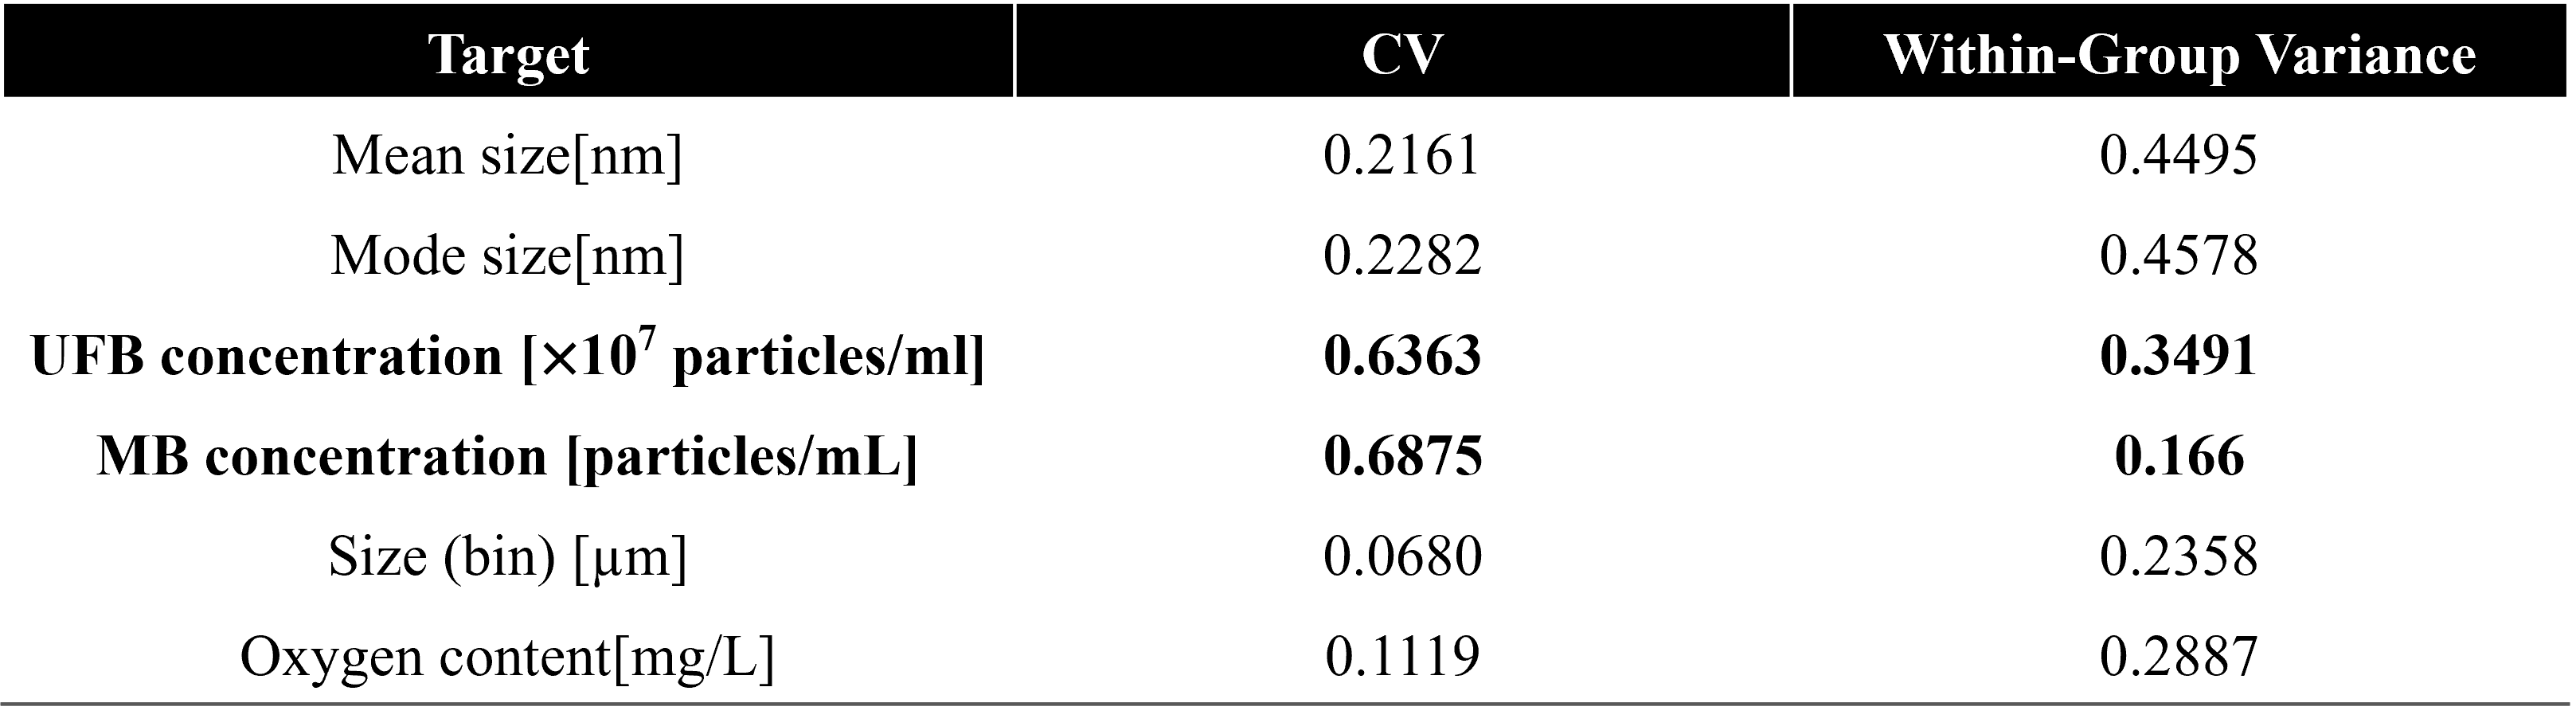
\includegraphics[width=\linewidth]{figures/table1_coefficient_of_variation_and_within_group_variance.png}
    \label{tab_cv}
\end{table}

選定した 3 つの目的変数と 6 つの説明変数について，各説明変数と目的変数の線形な関係の強さを把握するため，Pearson の積率相関係数を式(\ref{eq_pearson})により算出した．

\begin{equation}
    r_{e,t} = \frac{ \sum_{i=1}^{N} (x_i^e - \bar{x}^e)(y_i^t - \bar{y}^t) }{ \sqrt{ \sum_{i=1}^{N} (x_i^e - \bar{x}^e)^2 } \sqrt{ \sum_{i=1}^{N} (y_i^t - \bar{y}^t)^2 } }
    \label{eq_pearson}
\end{equation}

\noindent
ここで $ e $ は説明変数の種類，$ t $ は目的変数の種類，$ x_i^e $ は説明変数 $ e $ の $ i $ 番目のサンプルにおける値，$ y_i^t $ は目的変数 $ t $ の $ i $ 番目のサンプルにおける値，$ \bar{x}^e $，$ \bar{y}^t $ はそれぞれの平均，$ N $ はサンプル数である．
$ r_{e,t} $ は説明変数 $ e $ と目的変数 $ t $ の間の相関係数であり，$ -1 $ から $ 1 $ の値を取り，絶対値が大きいほど両変数間の線形な関係が強いことを示す．
なお，説明変数同士および目的変数同士の相関は本研究の関心対象外であるため算出していない．
図\ref{fig_correlation}に，算出した相関係数を示す．
Discharge tube は MB 濃度と負の相関（$ r = -0.46 $），酸素含量と正の相関（$ r = 0.65 $）を示し，操作条件の中で最も目的変数との関連が強い．
また，UFB 濃度は Flow speed (oxygen)（$ r = 0.38 $），Water volume（$ r = -0.40 $）とそれぞれ中程度の相関を示し，単一の説明変数に支配されない傾向がみられる．
このように，操作条件と目的変数の間に一定の線形相関が存在することから，操作条件から目的変数を予測する機械学習モデルの構築が有効であると考えられる．

\begin{figure}[H]
    \centering
    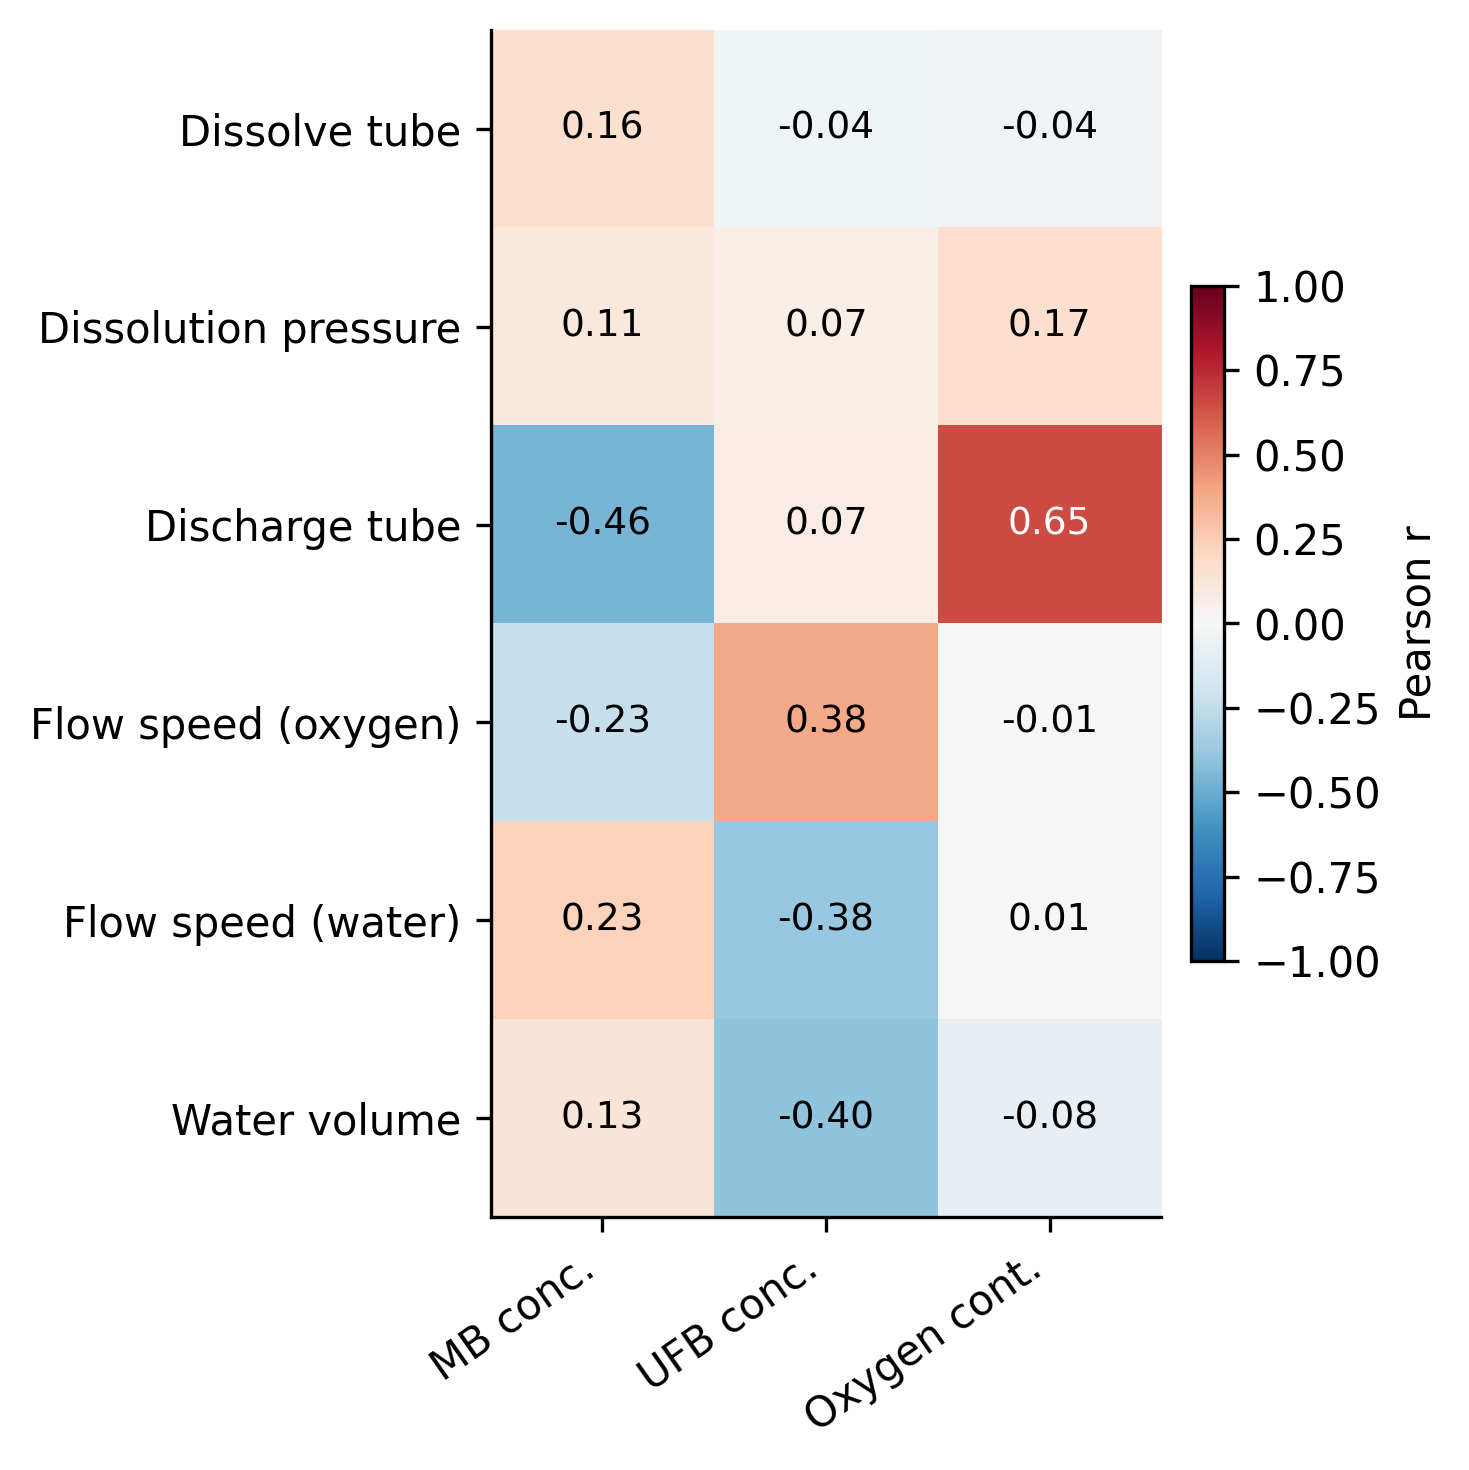
\includegraphics[width=\linewidth]{figures/figure2_correlation_coefficient.png}
    \caption{説明変数と目的変数の相関係数}
    \label{fig_correlation}
\end{figure}

\subsection{実験結果}
\label{sec_results}

選定した UFB 濃度，MB 濃度，酸素含量の 3 つの目的変数それぞれについて，説明変数から目的変数を予測する回帰モデルとして，線形回帰，多項式回帰，Random Forest の 3 種類を学習した．
線形回帰は 6 つの説明変数に対する線形結合により目的変数を予測するモデルであり，多項式回帰は各説明変数の 2 次の項および交互作用項まで拡張した上で線形回帰を適用するモデルである．
Random Forest は，学習データから復元抽出したサブサンプルおよび分岐候補となる説明変数をランダムに選択して構築した複数の決定木の予測値を平均する回帰モデルであり，本研究では決定木数を 100，各決定木の最大深さを 5 に設定した．

モデルの評価には，同一操作条件のサンプルが学習用データと評価用データに分かれて混入しないよう，操作条件を単位としてグループ化した 5-fold の Group $ k $-分割交差検証を用いた．
各モデルの予測誤差の指標には，式(\ref{eq_rmse})に示す平均二乗誤差平方根（Root Mean Squared Error，RMSE）を用いた．

\begin{equation}
    \mathrm{RMSE} = \sqrt{ \frac{1}{N} \sum_{i=1}^{N} \left( z_i - \hat{z}_i \right)^2 }
    \label{eq_rmse}
\end{equation}

\noindent
ここで $ z_i $ は標準化後の目的変数の真値，$ \hat{z}_i $ はモデルによる予測値，$ N $ はサンプル数である．
目的変数を標準化した上で RMSE を算出しているため，異なる目的変数間でも予測誤差の大きさを比較できる．

表\ref{tab_rmse}に，3 つの目的変数それぞれについて学習用データ（Train）および評価用データ（Test）に対する RMSE を示す．
いずれの目的変数についても Random Forest が最も低い Test RMSE を示し，3 つのモデルの中で最も高い予測性能を示した．
特に，多項式回帰は UFB 濃度において Train RMSE（$ 0.695 $）に対して Test RMSE（$ 1.168 $）が大きく上回っており，モデルが学習データに過剰適合している．
これは，6 つの説明変数を 2 次まで拡張したことでモデルのパラメータ数がサンプル数（82 サンプル）に対して相対的に多くなり，過学習が生じやすくなったためと考えられる．
一方，Random Forest は決定木の最大深さを制限した上で複数の決定木の予測を平均するため，Train RMSE と Test RMSE の乖離が 3 つのモデルの中で最も小さく，過学習が抑制されていることが確認できる．

\begin{table}[H]
    \caption{3 種のモデルによる目的変数ごとの Train／Test RMSE}
    \centering
    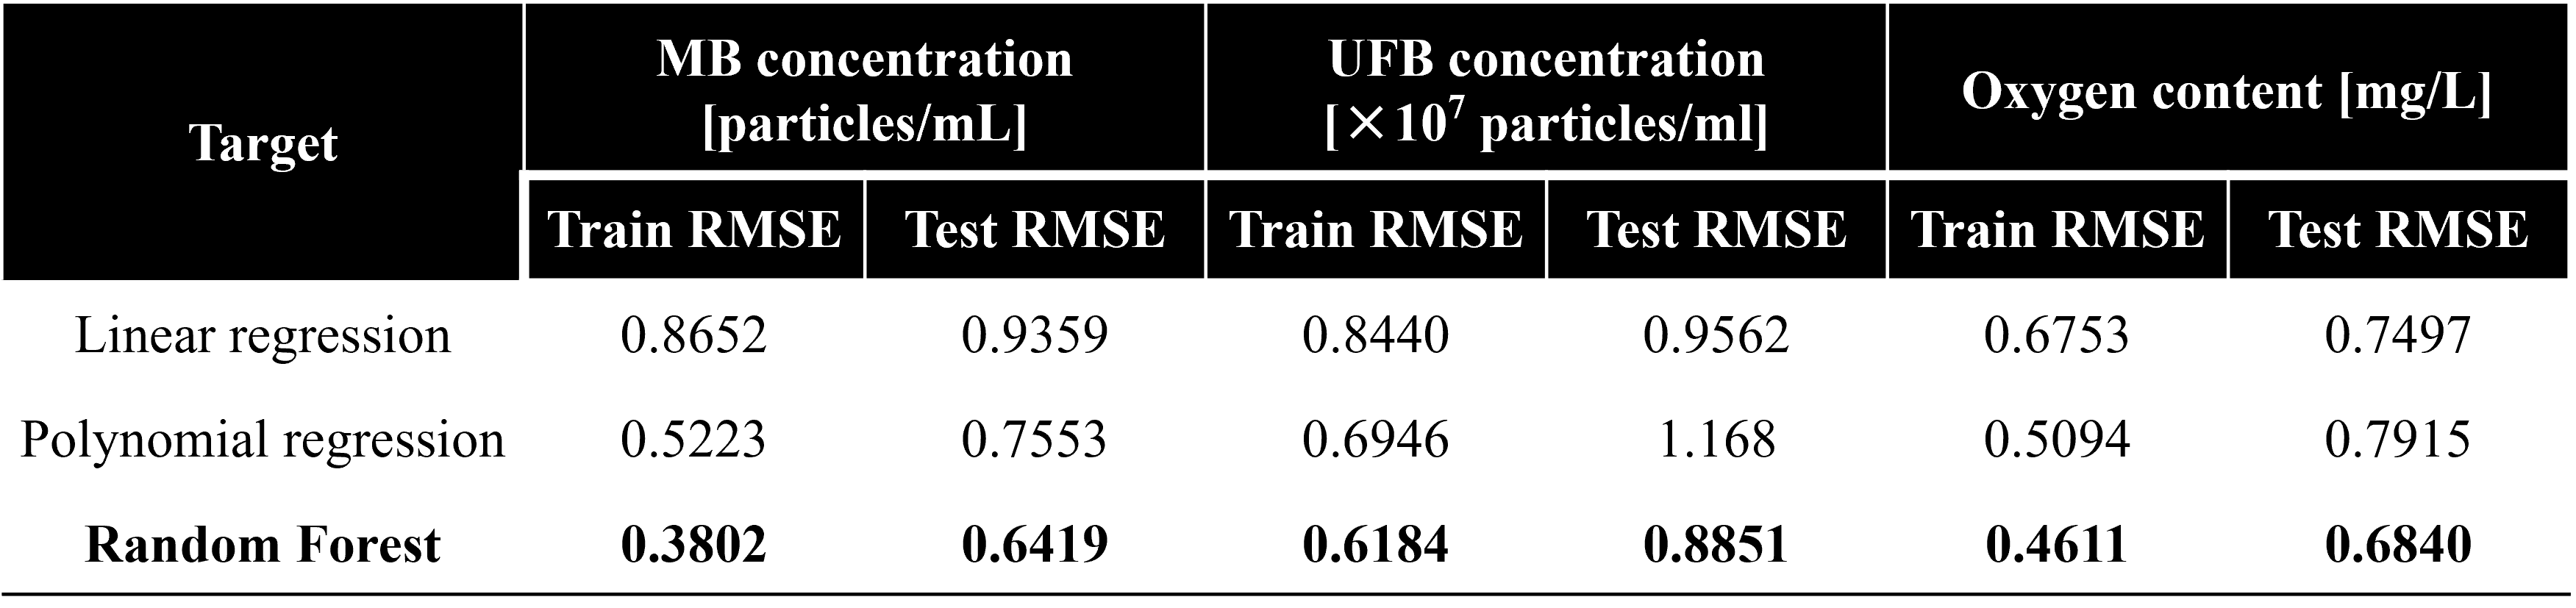
\includegraphics[width=\linewidth]{figures/table2_training_result.png}
    \label{tab_rmse}
\end{table}

Random Forest がどの説明変数を重視して予測を行っているかを分析するため，Mean Decrease in Impurity（MDI）に基づく Feature Importance を算出した．
本研究は回帰問題であるため，Feature Importance は式(\ref{eq_fi})に示す通り，森を構成する各決定木において，説明変数 $ j $ による分岐がもたらす二乗誤差の減少量を，その分岐に到達したサンプルの割合で重み付けして合計し，決定木数で平均した値として定義した．

\begin{equation}
    \mathrm{FI}_j = \frac{1}{T} \sum_{t=1}^{T} \sum_{v \in V_{t,j}} \frac{ n_v }{ n } \Delta e_v
    \label{eq_fi}
\end{equation}

\noindent
ここで $ T $ は決定木数，$ V_{t,j} $ は決定木 $ t $ において説明変数 $ j $ で分岐しているノードの集合，$ n_v $ はノード $ v $ に到達したサンプル数，$ n $ は全サンプル数，$ \Delta e_v $ はノード $ v $ における分岐前後の二乗誤差の減少量である．
本研究では，交差検証の各 fold で学習した Random Forest の Feature Importance を fold 間で平均した値を用いた．

図\ref{fig_fi} に，MB 濃度，UFB 濃度，酸素含量それぞれに対する Feature Importance を示す．

\begin{figure}[H]
    \centering
    \begin{subfigure}[b]{0.32\linewidth}
        \centering
        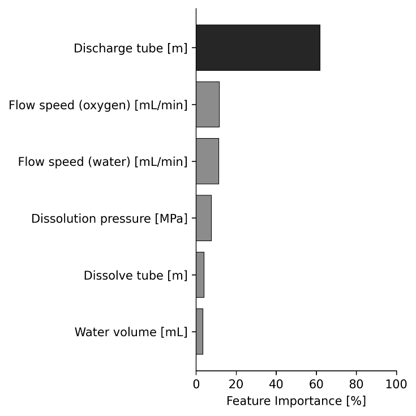
\includegraphics[width=\linewidth]{figures/figure3A_MB_feature_importance.png}
        \caption{MB 濃度}
        \label{fig_fi_mb}
    \end{subfigure}
    \hfill
    \begin{subfigure}[b]{0.32\linewidth}
        \centering
        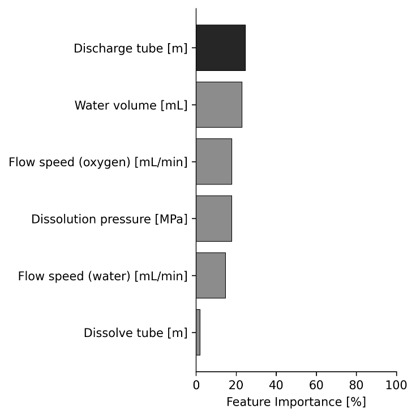
\includegraphics[width=\linewidth]{figures/figure3B_UFB_feature_importance.png}
        \caption{UFB 濃度}
        \label{fig_fi_ufb}
    \end{subfigure}
    \hfill
    \begin{subfigure}[b]{0.32\linewidth}
        \centering
        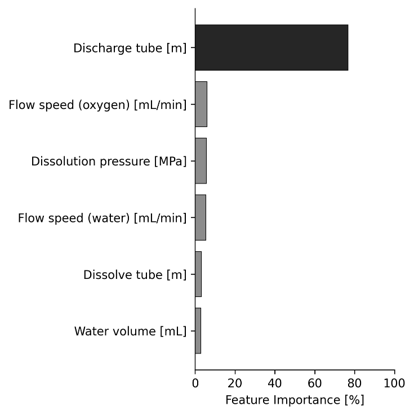
\includegraphics[width=\linewidth]{figures/figure3C_Oxygen_feature_importance.png}
        \caption{酸素含量}
        \label{fig_fi_oxygen}
    \end{subfigure}
    \par\vspace{2mm}
    \caption{目的変数ごとの Feature Importance}
    \label{fig_fi}
\end{figure}

図\ref{fig_fi}(A)および図\ref{fig_fi}(C)から，MB 濃度および酸素含量では，いずれも Discharge tube の Feature Importance が突出して高く（それぞれ約 $ 62\,\% $，約 $ 77\,\% $），単一の説明変数が支配的な重要度を示していることがわかる．
一方，図\ref{fig_fi}(B)から，UFB 濃度では Discharge tube が最も高い重要度を示すものの，Water volume，Flow speed (oxygen)，Dissolution pressure の重要度も同程度の水準にあり，特定の説明変数に支配されない分散した重要度分布となっていることがわかる．

3 つの目的変数のいずれにおいても Feature Importance が最大であった Discharge tube について，各水準における目的変数の分布を図\ref{fig_box}に箱ひげ図として示す．

\begin{figure}[H]
    \centering
    \begin{subfigure}[b]{0.32\linewidth}
        \centering
        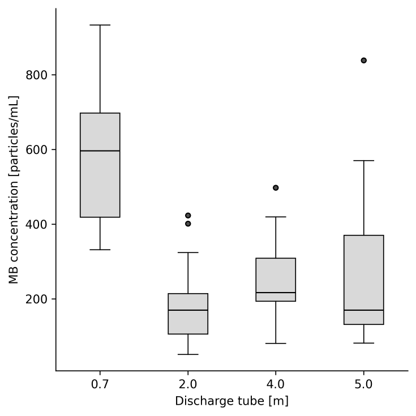
\includegraphics[width=\linewidth]{figures/figure4A_MB_box_plot.png}
        \caption{MB 濃度}
        \label{fig_box_mb}
    \end{subfigure}
    \hfill
    \begin{subfigure}[b]{0.32\linewidth}
        \centering
        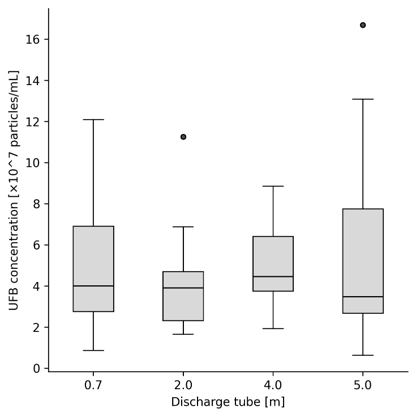
\includegraphics[width=\linewidth]{figures/figure4B_UFB_box_plot.png}
        \caption{UFB 濃度}
        \label{fig_box_ufb}
    \end{subfigure}
    \hfill
    \begin{subfigure}[b]{0.32\linewidth}
        \centering
        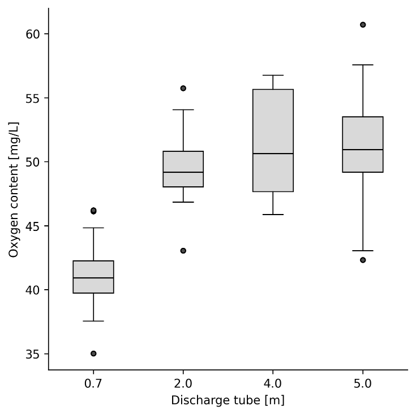
\includegraphics[width=\linewidth]{figures/figure4C_Oxygen_box_plot.png}
        \caption{酸素含量}
        \label{fig_box_oxygen}
    \end{subfigure}
    \par\vspace{2mm}
    \caption{Discharge tube と目的変数の関係}
    \label{fig_box}
\end{figure}

図\ref{fig_box}(A)から，MB 濃度は Discharge tube が $ 0.7\,\mathrm{m} $ で中央値が最も高く（約 $ 595 $），$ 2.0\,\mathrm{m} $ で最も低くなった後，$ 4.0\,\mathrm{m} $，$ 5.0\,\mathrm{m} $ にかけて分布が再び広がる非単調な関係を示すことがわかる．
図\ref{fig_box}(B)から，UFB 濃度は Discharge tube の各水準で中央値に明確な単調傾向はみられず，特に $ 5.0\,\mathrm{m} $ において分布の広がりが大きくなることがわかる．
図\ref{fig_box}(C)から，酸素含量は Discharge tube が長くなるにつれて中央値が単調に上昇する傾向を示す（$ 0.7\,\mathrm{m} $ で約 $ 41\,\mathrm{mg/L} $，$ 5.0\,\mathrm{m} $ で約 $ 51\,\mathrm{mg/L} $）ことがわかる．

\subsection{考察}
\label{sec_discussion}

表\ref{tab_rmse}に示した通り，Random Forest は 3 つの目的変数すべてにおいて線形回帰および多項式回帰よりも低い Test RMSE を示した．
この要因として，第一に，図\ref{fig_box}(A) に示した MB 濃度と Discharge tube の関係が挙げられる．
MB 濃度は Discharge tube が $ 0.7\,\mathrm{m} $ で最も高く，$ 2.0\,\mathrm{m} $ で低下した後，$ 4.0\,\mathrm{m} $，$ 5.0\,\mathrm{m} $ にかけて再び上昇する非単調な関係を示しており，このような関係は 1 次の項のみからなる線形回帰では表現できない．
Random Forest は決定木の分岐によって説明変数の値の範囲ごとに異なる予測値を割り当てることができるため，非単調な関係であっても近似が可能である．

第二に，多項式回帰は説明変数を 2 次まで拡張することで曲線的な関係をある程度表現できるものの，表\ref{tab_rmse}で確認した通り UFB 濃度において著しい過学習を示した．
これは，2 次の項および交互作用項への拡張によりパラメータ数が増加した結果，82 サンプルという限られたデータ数に対してモデルの表現力が過剰となったためと考えられる．
一方，Random Forest は決定木の最大深さを 5 に制限した上で 100 本の決定木の予測を平均するため，個々の決定木の過学習が緩和され，Train RMSE と Test RMSE の乖離が 3 つのモデルの中で最も小さく抑えられている．
以上より，操作条件と FB 物性値の関係が非線形かつ非単調であり，かつサンプル数が限られる本データセットにおいて，過学習を抑制しつつ非線形な関係を近似できる Random Forest が最も高い予測性能を示したと考えられる．

図\ref{fig_fi}および図\ref{fig_box}から，Discharge tube と目的変数の関係についてそれぞれ異なる特徴が読み取れる．

図\ref{fig_fi}(C)から，酸素含量は Discharge tube に対する Feature Importance が 3 つの目的変数中最も高い（約 $ 77\,\% $）ことがわかる．
図\ref{fig_box}(C)からも，Discharge tube の増加に伴って中央値が単調に上昇しており，相関係数（$ r = 0.65 $）とも整合する明確な単調増加の関係を示している．
このことから，酸素含量は Discharge tube という単一の操作条件によって説明できる度合いが高い目的変数であるといえる．

図\ref{fig_fi}(A)から，MB 濃度も Discharge tube の Feature Importance が高い（約 $ 62\,\% $）ことがわかるが，図\ref{fig_box}(A)に示した通り，Discharge tube との関係は単調ではなく，短い Discharge tube（$ 0.7\,\mathrm{m} $）と長い Discharge tube（$ 4.0$，$ 5.0\,\mathrm{m} $）の双方で分布が高い側に位置する．
相関係数（$ r = -0.46 $）が中程度の負の値にとどまっているにもかかわらず Feature Importance が高いのは，Feature Importance が線形な関係だけでなく非線形な関係も捉えられるためであり，MB 濃度と Discharge tube の間には線形相関では捉えきれない非単調な関係が存在することを示唆している．

これに対し，図\ref{fig_fi}(B)から，UFB 濃度は Discharge tube の Feature Importance が最も高いものの，Water volume，Flow speed (oxygen)，Dissolution pressure の Feature Importance も同程度の水準にあり，単一の説明変数に支配されないことがわかる．
この傾向は，\ref{sec_condition}節で述べた通り，各説明変数と UFB 濃度の相関係数がいずれも $ |r| \leq 0.4 $ 程度にとどまり，突出して大きい相関を示す説明変数が存在しないこととも整合する．
また，図\ref{fig_box}(B)においても，Discharge tube の各水準間で中央値に明確な傾向はみられず，特に $ 5.0\,\mathrm{m} $ で分布の広がりが大きくなっている．
以上のことから，UFB 濃度は Discharge tube 単独ではなく，複数の操作条件が複合的に影響することで決定される目的変数であると考えられる．

このように，本研究で対象とした 3 つの目的変数は，単一の操作条件（Discharge tube）で説明できる度合いが目的変数ごとに異なっており，特に酸素含量と MB 濃度については Discharge tube が支配的な要因である一方，UFB 濃度についてはより複合的な要因分析が必要であることが示唆された．


\end{document}
